58. а) Утверждение неверно, в качестве примера можно рассмотреть любой ромб (он описан, так как суммы противоположных сторон равны), не являющийся квадратом.\\
б) \begin{figure}[ht!]
\center{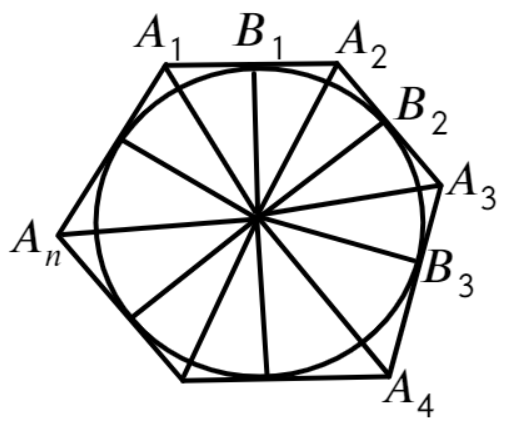
\includegraphics[scale=0.35]{g9-58.png}}
\end{figure}\\
Пусть углы многоугольника равны $\alpha.$ Соединим центр окружности $O$ со всеми вершинами и со всеми точками касания. Треугольники $OB_1A_2$ и $OB_2A_2$ равны по катету и гипотенузе, значит $B_1A_2=B_2A_2$ и $\angle B_1A_2O=\angle B_2A_2O=\cfrac{\alpha}{2}.$ Треугольники $OB_2A_3$ и $OB_3A_3$ также равны по катету и гипотенузе, значит $B_2A_3=B_3A_3$ и $\angle B_2A_3O=\angle B_3A_3O=\cfrac{\alpha}{2}.$ Но тогда треугольники $OA_2B_2$ и $OA_3B_2$ равны по катету и острому углу, поэтому $B_2A_2=B_2A_3.$ Проведя аналогичные рассуждения необходимое количество раз, получим, что все отрезки, на которые точки касания разбивают стороны, равны, а значит равны все стороны многоугольника, утверждение является верным.\\
